%04/02 - José Dorronsoro
\chapter{Programación dinámica}
\section{Revisando el problema del cambio}
Volvemos al problema de devolver el cambio de una cantidad de dinero. El algoritmo codicioso no siempre llegaba a la solución más óptima en cuanto a menor número de monedas devueltas. 
En este caso, el truco está en descomponer el problema en subproblemas y crear una fórmula para ir de un subproblema al siguiente.

Suponiendo que debemos dar un cambio C y tenemos las monedas $v_1 = 1, \ldots v_n$, entonces $n(i, c)$ es el número mínimo de monedas a cambiar utilizando solo las primeras $i$ monedas. Lo que queremos es $n(N, C)$, que se obtiene del subproblema $n(i, c)$. Además:
$$n(i,0) = 0$$
$$n(1,c) = c$$

Con esto, se puede rellenar una matriz con las monedas como filas y el posible cambio como columna. Para rellenar la posición $n(i,c)$:
\begin{itemize}
\item Si la moneda $i$ no entra en el cambio: $n(i - 1, c)$
\item Si la moneda $i$ sí entra en el cambio: $1 + n(i, c - v_i)$
\end{itemize}

\subsection{El algoritmo del cambio en programación dinámica}
De esta forma, llegamos a
$$n(i, c) = min{n(i - 1, c), 1 + n(i, c - v_i)}$$
con un coste $O(1)$.

En el problema, queríamos dar un cambio de 7 con monedas 1, 3, 4 y 5: $n(4, 7)$ Para ello, tenemos una tabla con las filas 1, 3, 4 y 5 y las columnas 0 1 2 3 4 5 6 7. La primera fila, con la moneda de 1, se rellena con el valor del cambio que hay que dar. Para la fila del 3, los valores de las columnas 0 1 y 2 se mantienen como la fila anterior, ya que no se puede utilizar esta moneda para un cambio menor a su valor. A partir del valor de la moneda, se debe retroceder ese valor en número de columnas y sumarle 1. Ese valor hay que compararlo con el de la celda justamente superior, y ver el valor mínimo, el cual se mantiene. Siguiendo esta lógica, llegamos a que el número de monedas mínimo para este problema son 2.

\begin{figure}[h]
\centering
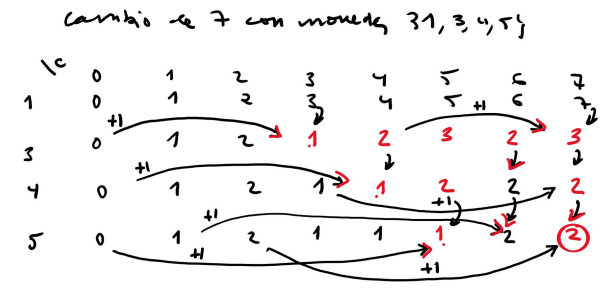
\includegraphics[width = 0.7\textwidth]{figs/dp-cambio.png}
\end{figure}

En este caso, hemos calculado $7 (c) \times 4 (n) = 28$ veces. El coste de un algoritmo sin bucles es constante: $f(n) = 1$. Por tanto, en este caso el coste es $28 \times O(1)$, y de forma general:
$$N \times C \times O(1) = O(N \times C) = O(N \times 2^{logC})$$
siendo $2^{logC}$ el logaritmo binario de C (los bits en los que se puede codificar).

\section{Algoritmos de cadenas en programación dinámica}
Para un informático, una secuencia biológica son cadenas de texto.
Teniendo dos cadenas, para transformar una en la otra, se puede:
\begin{itemize}
\item Cambiar un caracter por otro
\item Insertar un caracter
\item Borrar un caracter
\end{itemize}
Insertar un caracter en una cadena es equivalente a borrar un caracter en la otra. Además, queremos mantener una cadena constante y modificar solo la otra. 

La \textbf{distancia de edición} entre dos cadenas es el número mínimo de de operaciones de edición que se deben hacer para convertir una en la otra. 

Dados los strings S y T con M y N número de caracteres respectivamente,se consideran los substrings  
$$S_i = [s_1, \ldots s_i]$$
$$T_i = [t_1, \ldots t_j]$$

Así, $d_{i,j}$ es la distancia de edición entre $S_i$ y $T_i$. Si $s_i = t_j$, entonces $d_{i,j} = d_{i-1, j-1}$, ya que la diferencia se encuentra antes. Si $s_i \neq t_j$, hay tres opciones:
\begin{itemize}
\item Cambiar $t_j$ por $s_i$; entonces $d_{i,j} = 1 + d_{i-1, j-1}$
\item Borrar $t_j$ de $T_j$; entonces $d_{i,j} = 1 + d_{i, j-1}$
\item Borrar $s_i$ de $S_i$; entonces $d_{i,j} = 1 + d_{i-1, j}$
\end{itemize}
De estas tres opciones, se calculan todas y nos quedamos con el mínimo.

\subsection{Rellenar la matriz}
Tenemos una matriz con M filas y N columnas. Esto se multiplica por lo que cuesta calcular cada elemento, O(1): $O(M \times N)$. Esto es caro en tiempo y en memoria. 

Finalmente, tenemos las siguientes ecuaciones para el problema de la distancia de edición:
$$d_{i,j} = \begin{cases}
d_{i-1, j-1} & \text{cuando} s_i = t_j \\
1 + min {d_{i-1, j-1}, d_{i, j-1}, d_{i-1, j}} & \text{cuando} s_i \neq t_j
\end{cases} $$

Ejemplo: encontrar la distancia de edición entre \texttt{biscuit} y \texttt{suitcase}.
\begin{figure}[h]
\centering
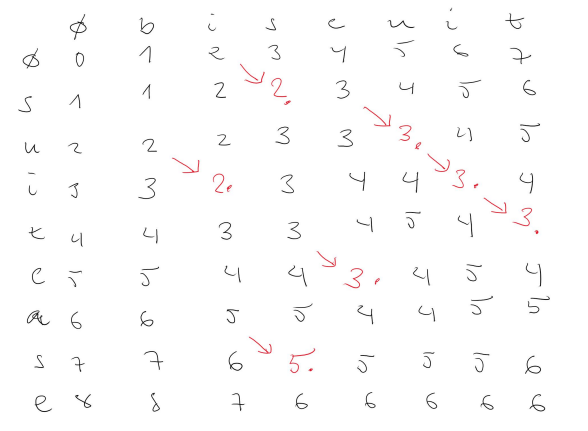
\includegraphics[width = 0.6\textwidth]{figs/edit-distance-ex.png}
\end{figure}

No obstante, en biología, se asignan costes a cambiar y a borrar diferentes dependiendo del caso.
